\documentclass{beamer}
\usetheme{default}
\usecolortheme{seahorse}
\usepackage[utf8]{inputenc}
\usepackage{graphicx}
\usepackage{booktabs}
\usepackage{amsmath}
\usepackage{natbib}
\usepackage[italian]{babel}
\usepackage{hyphenat}
\hyphenation{mate-mati-ca recu-perare}
\usepackage{tikz}
\usetikzlibrary{shapes,arrows.meta,positioning}

\title[Lezione 1]{Hello, Psychometrics!}
\subtitle{Master Avanzato in Economia e Politica Agraria}
\author{Giovanbattista Califano}
\date[Portici, 20/04/2026]{Scale Attitudinali per lo Studio \\ delle Preferenze del Consumatore \\ 20 Aprile 2026}
\institute[UNINA]{Università degli Studi di Napoli Federico II, giovanbattista.califano@unina.it}

\AtBeginSection[]
{
  \begin{frame}<beamer>
    \frametitle{Passiamo a...}
    \tableofcontents[currentsection]
  \end{frame}
}

\begin{document}

\frame{\titlepage}

\begin{frame}{Tabella di marcia}
    \begin{center}
        \begin{tabular}{|l|l|c|}
        \hline
        20/04 &  Hello, Psychometrics! & $\bigcirc$ \\
        \hline
        23/04 &  Il Questionario & $\bigcirc$ \\
        \hline
        24/04 & Affidabilità e Validità di una Misura & $\bigcirc$ \\
        \hline
        27/04 & Variabili Latenti: Riflessive o Formative? & $\bigcirc$ \\
        \hline
        30/04 & Un po' di SEM & $\bigcirc$ \\
        \hline
        07/05 & Stata Stata Stata Stata Stata Stata Stata & $\bigcirc$ \\
        \hline
        \end{tabular}
    \end{center}
\vspace{0.1cm}
\footnotesize
Riferimenti consigliati: \\
\begin{itemize}
    \item Capitoli 4 e 7 da \cite{jhangiani2019research}
    \item Capitoli 7, 10 e 14 da \cite{olivero2022psicologia}
    \item Capitolo 12 da \cite{mehmetoglu2022applied}
\end{itemize}
\scriptsize
\bibliographystyle{apalike}
\bibliography{text}
\end{frame}

\begin{frame}{Perché la psicometria? Il caso del dott. Mirko Marmellata}
\begin{figure}
    \centering
    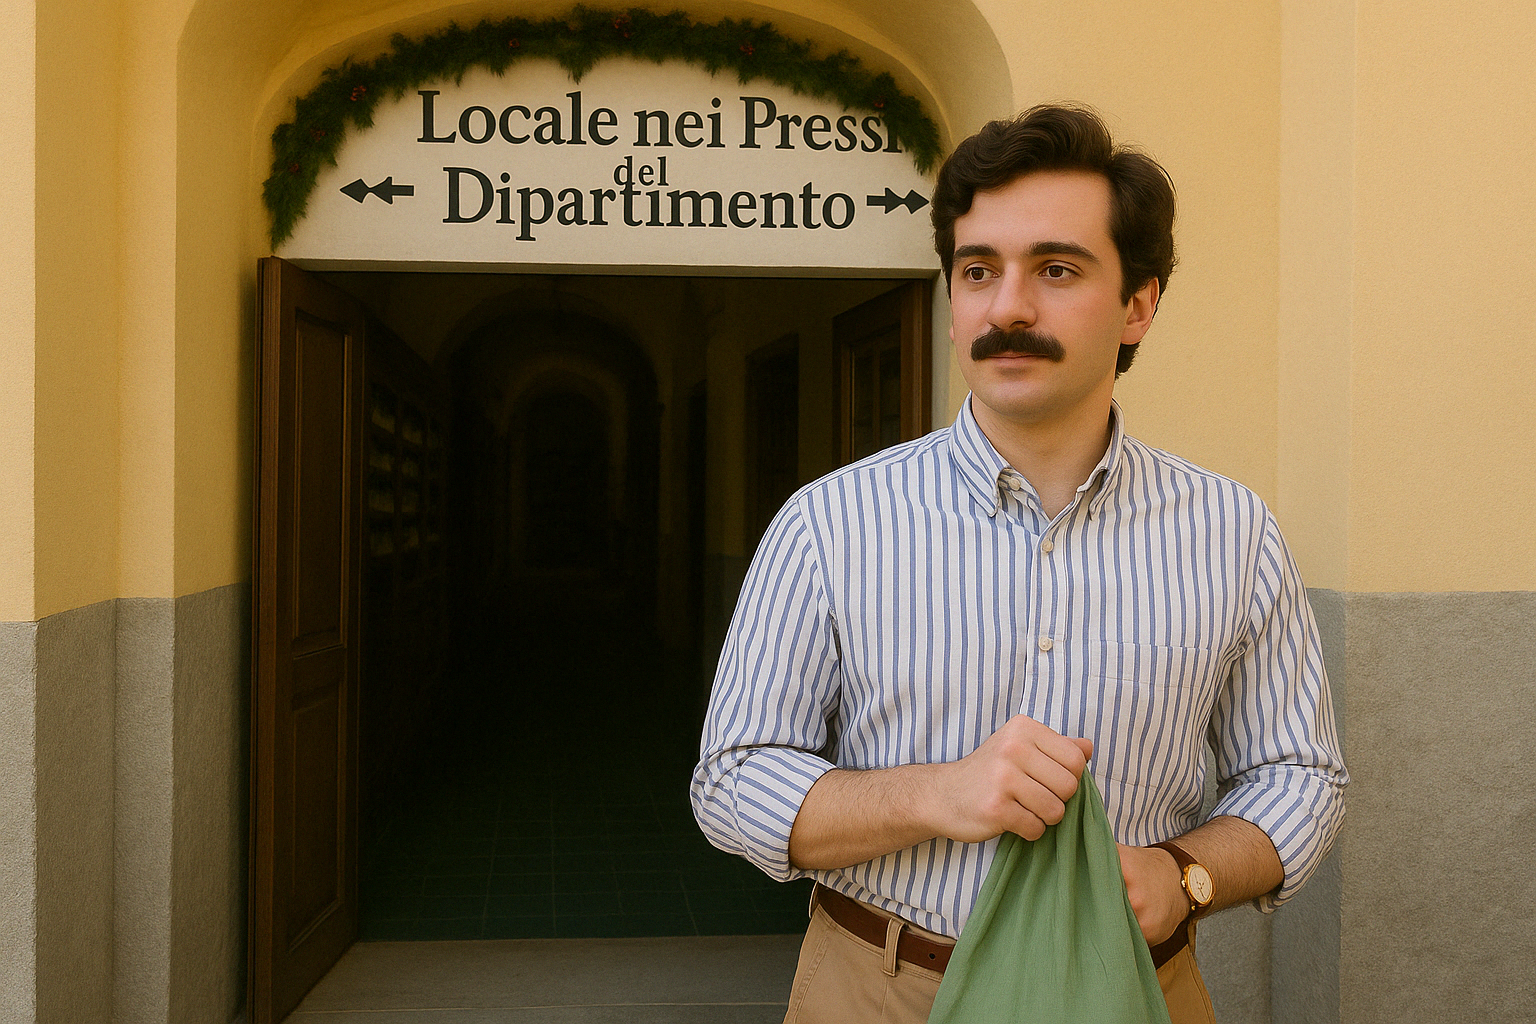
\includegraphics[width=\linewidth]{mirko.png}
\end{figure}
\end{frame}

\begin{frame}{Perché la psicometria? Il caso del dott. Mirko Marmellata}
\begin{block}{Il dott. Marmellata}
ogni giorno sceglie di comprare il pranzo al \textit{Locale nei Pressi del Dipartimento}, nonostante spenda molto di più rispetto al portarsi il pranzo da casa, e non sia mai del tutto soddisfatto della qualità e della quantità offerta.
\end{block}
\vspace{1em}
\begin{block}{Per gli standard dell'homo oeconomicus}
la sua scelta sarebbe \textbf{irrazionale}. Volendo essere gentili, la scelta ci appare comunque \textbf{non ottimale}.
\end{block}
\end{frame}

\begin{frame}{Perché la psicometria? Il caso del dott. Mirko Marmellata}
\begin{block}{Random Utility Model (RUM)}
\[
U_{ia} = V_{ia} + \varepsilon_{ia}
\]
\begin{itemize}
  \item \(U_{ia}\): utilità totale che l’individuo \(i\) associa all’alternativa \(a\);
  \item \(V_{ia}\): componente osservabile (prezzo, quantità...);
  \item \(\varepsilon_{ia}\): componente non osservata (abitudini, emozioni...).
\end{itemize}
\end{block}
\vspace{1em}
\begin{block}{Per Mirko Marmellata:}
\[
U_{\text{MM}, \text{Locale}} > U_{\text{MM}, \text{Casa}}
\]
Ciò che guida la sua preferenza è probabilmente nascosto in \(\varepsilon\).
\end{block}
\end{frame}

\begin{frame}{Perché la psicometria? Il caso del dott. Mirko Marmellata}
\begin{block}{Il ruolo della psicometria}
Permette di ``aprire'' la \(\varepsilon\) e di modellare i costrutti latenti che influenzano le decisioni.
\end{block}
\vspace{1em}
\begin{block}{Obiettivo}
Portare i fattori psicologici fuori da \(\varepsilon\) e dentro il modello, migliorando \textbf{predizione} e \textbf{comprensione}.
\end{block}
\end{frame}

\section{Breve introduzione alla teoria della misurazione}
\begin{frame}{Vietnam flashback...}
\begin{center}
   {\huge \alert{DATA GENERATING PROCESS}} 
\end{center}
\vspace{0.5cm}
\begin{itemize}
    \item Come misurare qualcosa che non possiamo osservare?
\end{itemize}
\pause
\vspace{0.5cm}
Secondo la \textbf{teoria della misurazione}, anche se non possiamo osservare direttamente un concetto teorico (come l'intelligenza), possiamo osservarne i {\it riflessi} nella realtà: comportamenti, risposte, risultati... \\
\vspace{0.5 cm}
\footnotesize
{\it Esempio:} \\
Non pesiamo l'intelligenza di una persona su una bilancia, ma possiamo inferirla da una serie di segnali: si è laureata con lode, è brava con Stata, usa parole complicate, ha letto tutti i romanzi russi dell'Ottocento... {\it Nota che molto dipende dalla nostra definizione di intelligenza!}
\end{frame}

\begin{frame}{Cosa intendiamo per misurazione}
\begin{block}{Definizione proposta:}
    Assegnazione \textit{sitematica} di un punteggio a delle entità (individui, oggetti, eventi...), in modo tale che il punteggio rappresenti una caratteristica di quelle entità.
\end{block}
\pause
\begin{itemize}
    \item Quando la caratteristica investigata è di natura psicologica, la scienza della misurazione è chiamata \textbf{psicometria}.
\end{itemize}
\end{frame}

\section{I costrutti: definizioni concettuali e operazionali}
\begin{frame}{I costrutti}
Alcune caratteristiche di interesse sono semplici da misurare: età del consumatore, altezza, peso. \\ Altre, come l’intelligenza, l’autostima o gli atteggiamenti, non possono essere osservate direttamente.
\begin{itemize}
    \item Queste variabili si chiamano \textbf{costrutti}.
\end{itemize}
\end{frame}

\begin{frame}{I costrutti}
I costrutti includono (ma non si limitano a):
    \begin{itemize}
      \item Tratti di personalità (es. estroversione)
      \item Stati emotivi (es. paura)
      \item Atteggiamenti (es. verso le certificazioni)
      \item Abilità (es. nelle materie scientifiche)
    \end{itemize}
\end{frame}

\begin{frame}{I costrutti}
  \begin{itemize}
    \item Il costrutto descrive una \textit{tendenza generale} ad agire in un certo modo, non un comportamento specifico nel momento.
    \item I costrutti sono \textbf{sintesi astratte} di processi complessi.
    \item Nessun comportamento o processo singolo può “definire” completamente il costrutto.
  \end{itemize}
\end{frame}

\begin{frame}{Definizione concettuale di un costrutto}
  \begin{block}{Cos'è una definizione concettuale?}
    Descrive i comportamenti e i processi interni che costituiscono un costrutto psicologico, e spiega come esso si relaziona ad altre variabili.
  \end{block}
  \pause
  \begin{itemize}
    \item Esempio: il \textbf{neuroticismo} può essere definito come la tendenza stabile a provare emozioni negative (ansia, rabbia, tristezza) in molteplici situazioni.
    \item Può includere anche: origine genetica, stabilità nel tempo, correlazioni con dolore fisico e sintomi somatici.
    \pause
    \item Le definizioni scientifiche differiscono da quelle del dizionario (più precise, empiricamente testabili, e aperte alla revisione).
    \item Spesso esistono più definizioni concettuali dello stesso costrutto in letteratura.
  \end{itemize}
\end{frame}

\begin{frame}{Definizione operazionale di un costrutto}
  \begin{block}{Cos'è una definizione operazionale?}
    È una definizione di un costrutto in termini di come viene misurato concretamente.
  \end{block}
  \pause
\vspace{0.8cm}
  \begin{center}
      \textbf{Definizione concettuale} \\
      \bigskip
      $\Downarrow$ \quad \textit{\small Operazionalizzazione} \quad $\Downarrow$ \\
      \bigskip
      \textbf{Definizione operazionale} \\
  \end{center}
\end{frame}

  
\begin{frame}{Definizione operazionale di un costrutto}
  Le misure operazionali si dividono in tre grandi categorie:
  \begin{enumerate}
      \item \textbf{Self-report}: l'individuo riporta i propri pensieri, emozioni o comportamenti.
      \item \textbf{Comportamentale}: si osserva e registra un comportamento.
      \item \textbf{Fisiologica}: si registrano processi biologici.
    \end{enumerate}
\end{frame}

\begin{frame}{Esempio: Risposta di disgusto verso uno yogurt “scaduto"}
\small
  Supponiamo di voler misurare la reazione di \textbf{disgusto} di un consumatore verso uno yogurt che ha superato il termine minimo di conservazione.
  \pause
      \begin{block}{Definizione concettuale}
    Il disgusto è un'emozione di base che si manifesta come risposta di evitamento verso stimoli percepiti come contaminanti, infetti o degradati. Ha una funzione evolutiva di protezione dall'ingestione di sostanze potenzialmente pericolose.
  \end{block}
  \pause
    \begin{block}{Definizioni operazionali}
  \begin{itemize}
    \item \textbf{Self-report}: il partecipante valuta quanto trova disgustosa l'idea di assaggiare il prodotto su una scala da 1 a 7.
    \item \textbf{Comportamentale}: si osserva se il partecipante rifiuta di assaggiare il prodotto.
    \item \textbf{Fisiologica}: si misura la risposta galvanica della pelle (GSR) o l'attività muscolare facciale (EMG) legata al disgusto quando chiediamo al partecipante di assaggiare il prodotto.
  \end{itemize}
\end{block}
\end{frame}

\section{I livelli di misurazione}
\begin{frame}{Livelli di misurazione}
  \begin{block}{Il livello della misurazione può essere:}
    \begin{enumerate}
      \item Nominale
      \item Ordinale
      \item A intervalli
      \item A rapporti
    \end{enumerate}
 \end{block}
Ogni livello comunica un diverso grado di informazione quantitativa, e ne determina le analisi statistiche appropriate.
\end{frame}

\begin{frame}{Nominale e Ordinale}
\begin{block}{Nominale}
    Etichette di categoria: es. genere, stato civile, etnia, colore preferito. \textbf{Non c'è nessun ordine tra le categorie.}
\end{block}
\pause
\begin{block}{Ordinale}
    Le categorie hanno un ordine (es. “molto soddisfatto", “soddisfatto", “insoddisfatto") \textbf{ma non è possibile assumere che le distanze tra le categorie siano uguali.} \\
    \pause
    \centering
    \vspace{0.5em}
    \begin{tikzpicture}[x=2cm,y=1cm]
  \fill[blue!30] (-1,-0.1) rectangle (0,2.2);     
  \fill[blue!70] ( 0,-0.1) rectangle (1,3.0);     
  \fill[blue!10] ( 1,-0.1) rectangle (2,1.5);     
  \node[font=\large\bfseries] at (-0.5,1.1) {2};
  \node[font=\large\bfseries] at ( 0.5,1.8) {1};
  \node[font=\large\bfseries] at ( 1.5,0.75) {3};
\draw[thick] (-1,-0.1) -- (2,-0.1);
    \pause
  \node at (-0.5,2.6) {01:00:26};
  \node at ( 0.5,3.4) {00:59:42};
  \node at ( 1.5,1.9) {01:00:37};
\end{tikzpicture}
\end{block}
\end{frame}

\begin{frame}{A Intervalli e a Rapporti}
  \begin{block}{A Intervalli}
  Differenze numeriche con significato coerente: es. gradi Celsius. \\
  La distanza tra 12°C e 22°C è la stessa che separa 22°C da 32°C. Però...
    \begin{itemize}
      \item \textbf{Nessun vero zero:} 0°C non significa “assenza di temperatura".
      \item Quindi \textbf{non ha senso parlare di “doppio” o “metà”:} a 30°C non fa il doppio del caldo di 15°C.
    \end{itemize}
  \end{block}
  \pause
  \begin{block}{A Rapporti}
  Come gli intervalli, ma con lo zero che indica l'\textbf{origine assoluta}. \\
    \begin{itemize}
      \item Permette confronti di proporzione: 100 kg è il doppio di 50 kg.
      \item Es.: altezza, peso, reddito, temperatura in Kelvin.
    \end{itemize}
  \end{block}
\end{frame}

\begin{frame}{Ricapitolando}
    \centering
    Operazioni possibili con le diverse scale di misura: \\
    \vspace{1em}
    \begin{tabular}{lcccc}
    \toprule
      \textbf{Livello} & \textbf{$=$ $\neq$} & \textbf{$>$ $<$} & \textbf{$+$ $-$} & \textbf{$\times$ $\div$} \\
      \midrule
      Nominale & \checkmark & & & \\
      Ordinale & \checkmark & \checkmark & & \\
      A Intervalli & \checkmark & \checkmark & \checkmark & \\
      A Rapporti & \checkmark & \checkmark & \checkmark & \checkmark \\
      \bottomrule
    \end{tabular}
\end{frame}
\end{document}